\chapter{Toward A Thousand Lights: Decentralized Deep ReinforcementLearning for Large-Scale Traffic Signal Control}
\label{chap:thousand}

\section{Preliminaries}
 
\begin{definition}[Traffic movement]
A traffic movement is defined as the traffic traveling across an intersection from one entering lane to an exiting lane. We denote a traffic movement from road $l$ to road $m$ as $(l,m)$. 
% We call $m$ is the downstream lane of $l$ and denote all the downstream lanes of $l$ as $Out_l$.
\end{definition}

\begin{definition}[Pressure of traffic movement]
Denote by $x(l,m)$ the number of vehicles for traffic movement $(l,m)$, the pressure of a traffic movement, $p(l,m)$ is simplely the difference between $x(l,m)$ and the average number of vehicles for all $l$'s downstream lanes.
    \end{definition}

% \chacha{Figure of MFD Fixedtime control}

\begin{problem}[Multi-intersection traffic signal control]
Each intersection is controlled by an RL agent. At time step $t$, agent $i$ views part of the environment as its observation $o^t_i$. Given the traffic situation and current traffic signal phase, the goal of the agent is to take an optimal action $a$ (i.e., which phase to set), so that the cumulative reward $r$ can be maximized. 
\end{problem}

% !TEX root = main.tex
\begin{figure}[t!]
\centering
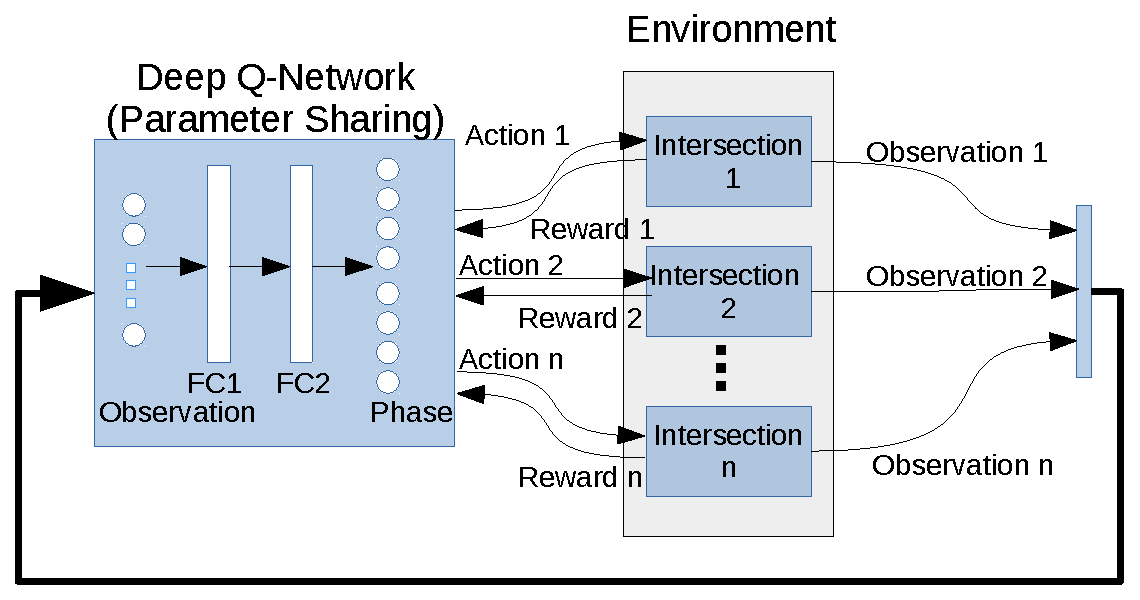
\includegraphics[width=.46\textwidth]{figures/framework.pdf}
%\vspace{-2mm}
\caption{The framework of \PressLight for multi-intersection signal control.}%\vspace{-2mm}
\label{fig:framework}
\end{figure}


\section{Method}
% We propose the decentralized reinforcement learning approach \PressLight for multi-intersection signal control. 

In this section, we first introduce the basic elements for reinforcement learning and describe the motivation of our novel reward design. Then we present the proposed \PressLight as a typical Deep Q-Network agent and show its learning process, as Figure~\ref{fig:framework} illustrates. For large-scale network signal control, we leverage parameter sharing among the agents, as discussed in the last part.

\begin{figure}[t!]
\centering
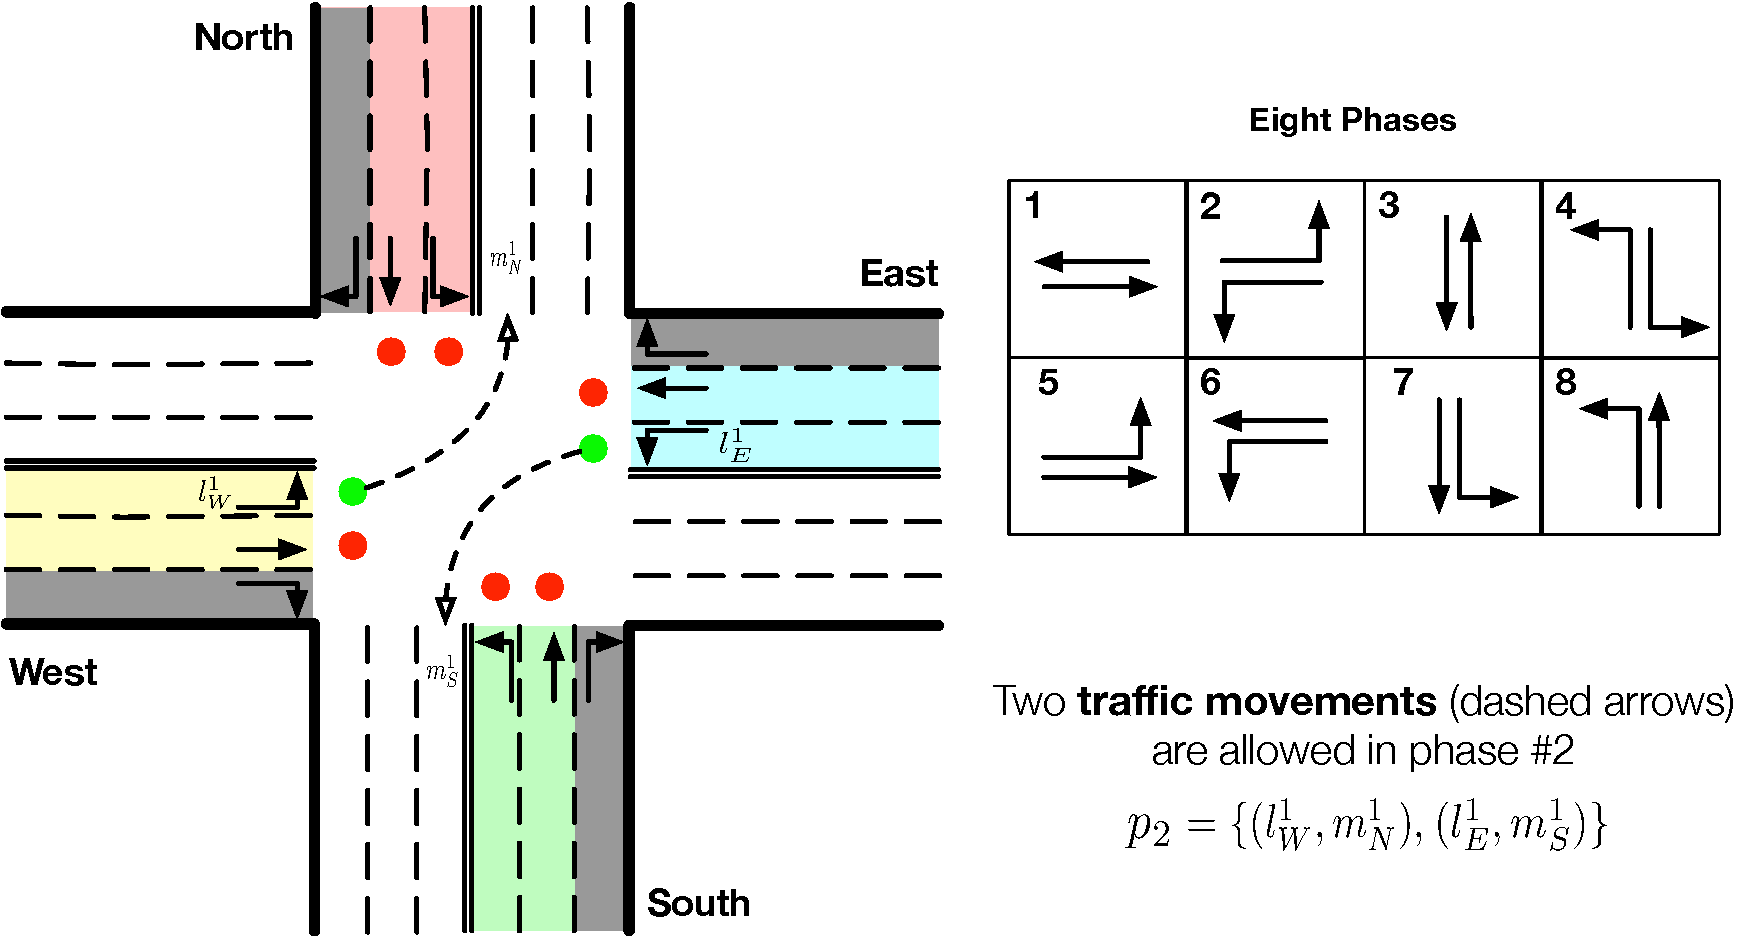
\includegraphics[width=0.36\textwidth]{figures/phase_detail.pdf} 
%\vspace{-2mm}
\caption{The illustration of an intersection with eight phases. In this case, phase \textbf{\#2} is set.}
%\vspace{-2mm}
\label{fig:phase}
\end{figure}

% Each intersection is controlled by an RL agent. An agent can only observe the local traffic situation (i.e. the traffic situation on all its entering and exiting approaches) and control the traffic signal accordingly. The goal of the agent is to learn a policy which maximizes its own long term cumulative reward.

% \subsection{Generic Model}
\subsection{Agent Design}
We design the state, the action as well as the reward for the \PressLight agent as follows.

\begin{itemize}
    \item \textbf{Observation}. Each agent observes part of the system state as its own observation. For a standard intersection with 12 traffic movements, its observation includes the current phase $p$ and the pressure of the 12 traffic movements. Note that for the intersection with fewer than 12 movements, the vector is zero-padded\footnote{In this paper, we only consider no more than 12 traffic movements, but the proposed method can be easily extend to control intersections with more than 12 movements.}.
    \item \textbf{Action}. 
         At time $t$, each agent chooses a phase $p$ as its action $a_t$, indicating the traffic signal should be set to phase $p$. 
         As shown in Figure~\ref{fig:phase}, eight phases are used to control the traffic movements in each intersection. For example, when phase \#2 is activated, the vehicles on the left-turn lane on the East and the West are allowed to turn left to their corresponding exiting lanes.
         
        %  Define agent (intersection) $i$'s action set as\\
        %  $A_i = \{(l,m) \text{for all the permissible traffic movement}\}$, 
         
        %  \WEs (going Straight from West and East), \SNs (going straight from South and North), \WEl (turning left from West and East), \SNl (turning left from South and North), \WW (going straight and turning left from West), \NN(going straight and turning left from North), \EE(going straight and turning left from East), \SSl(going straight and turning left from South).  


    %  At time $t$, each agent chooses a phase $p$ as its action $a_t$, indicating the traffic signal should be set to phase $p$. In our environment, Each action candidate $a_{i}$ is an one-hot vector representing a phase. 

    % Note that without loss of generality, in the grid road net setting, the set of actions only includes 4 phases while in the real-world scenario, it includes all the 8 phases. 


    \item \textbf{Reward}. In Figure~\ref{fig:pressure}, we define the reward $r_i$ for agent $i$ as the pressure on the intersection, which is simply the difference between the sum of the queueing vehicles on all the entering lanes and the sum of the queueing vehicles on all the exiting lanes.
    
    If we denote the pressure of intersection $i$ by $P_i$ , then the reward $r_i$ should be
        \begin{equation}
            \label{eq:reward-detail}
            r_i  = - P_i.
        \end{equation}
    By maximizing the reward, the agent is trying to stabilizing the queues in the system.
    \begin{figure}[htbp]
        \centering
        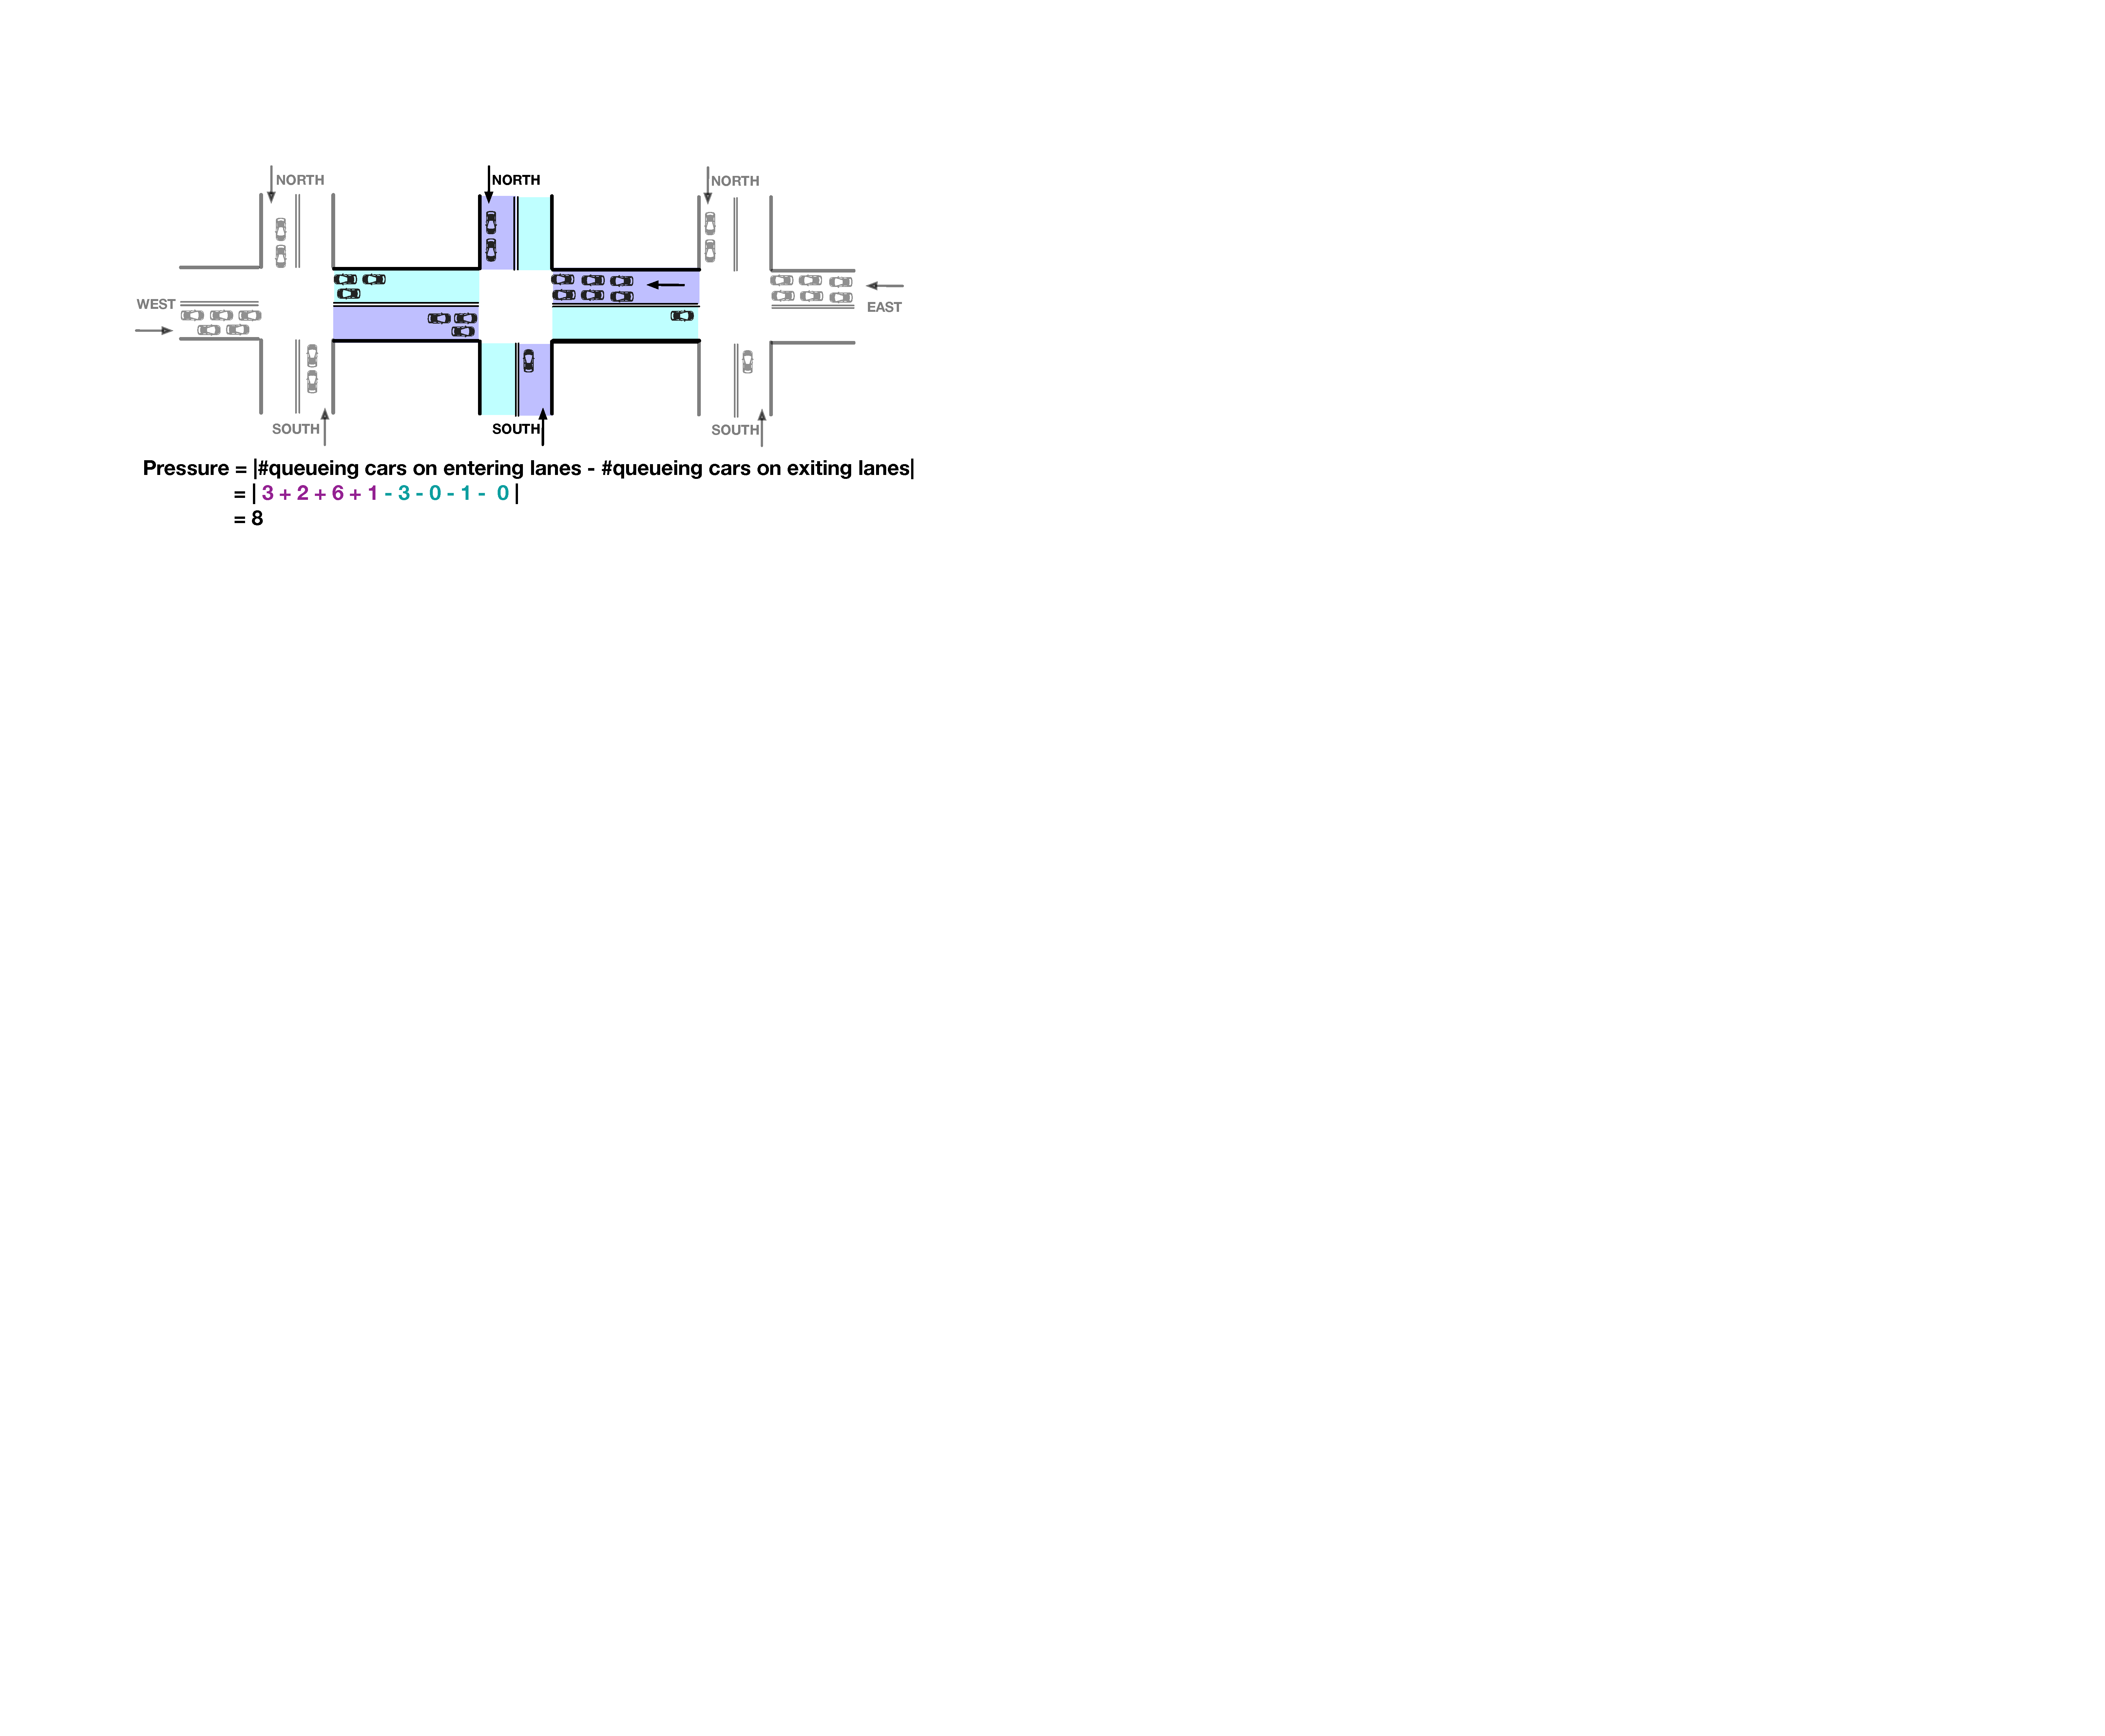
\includegraphics[width=0.5\textwidth]{figures/pressure_def.pdf} %\vspace{-2mm}
        \caption{The illustration of intersection pressure.}%\vspace{-2mm}
        \label{fig:pressure}
        \end{figure}
    % Intuitively, the By minimizing, the vehicles within the system can be evenly distributed. Then the green light is effectively utilized so that the throughput is optimized.
    % If we regard all the intersections have the same maximum capacity $x_{max}$ and $x(l,m)^{down}=\sum_{p\in Out_m}{r(m,p)\cdot x(m,p)}$ as the downstream number of vehicles and $x(l,m)$ as the upstream number of vehicles, then 
    % \begin{equation}
    % w(l,m)= x(l,m)-x^{down}(l,m)
    % \end{equation}
    % is simply \textit{the difference between the upstream and downstream number of vehicles}. If the vehicles are not allowed to change their lanes, then $|Out_m|=1$ and $r(m,p)=1$, we have $w(l,m)= x(l,m)-x(m,p)$, which is simply the difference of number of vehicles between the upstream and downstream lane.
\end{itemize}


\subsection{Reward Function Verification}
In previous work~\cite{varaiya2013max}, max pressure control law utilized only local information at each intersection under infinite capacities and has been proved to be stability-optimal, i.e., stabilizing and maximizing the throughput. In practice, however, max pressure control is often implemented in a greedy manner, which leads to a local optimum, see Algorithm~\ref{alg:mp}.
% Basically, max pressure control greedily searches the phase to set which minimize the pressure of an intersection.
% Our reward design match the objective of max pressure control law. Each individual agent maximizes its own reward.


\begin{algorithm}[H]
% \SetAlgoLined
% \KwResult{Write here the result }
%  initialization\;
\For{each intersection $i$}{
\For{each traffic movement (l,m)}
{   
calculate $p(l,m)$
}
next phase $\leftarrow \arg\max \{p(l,m) |\text{if $(l,m)$ is permissible} \} $ 

}


%  \While{While condition}{
%   instructions\;
%   \eIf{condition}{
%   instructions1\;
%   instructions2\;
%   }{
%   instructions3\;
%   }
%  }
 \caption{Max Pressure Control}
 \label{alg:mp}
\end{algorithm}


By setting the reward of our RL agents to be the same as max pressure control objective, each local agent is maximizing its own cumulative reward, which further maximizes the network throughput under certain constraints.



%  The key idea of MP is to minimize the ``pressure'' of an intersection., which can be loosely defined as number of vehicles on entering lane minus the number of vehicles on exiting lane. Figure~\ref{fig:pressure} illustrates the concept of pressure. By setting the objective as minimizing the pressure of intersections, MP is proved to maximize the throughput of the whole road network\footnote{Maximizing throughput equals to minimizing travel time under certain conditions and minimizing travel time is the final goal for traffic signal control.}. However, the solution of MP is greedy which leads to locally optimal solutions. 
 
%  \chacha{todo}
 


% MARL with parameter sharing network
% because all the agent should ultimately converge upon the same value function

\subsection{Deep Q-learning}
As shown in Figure~\ref{fig:framework}, we use a Deep Q-Network (DQN) to solve the multi-intersection signal control problem. Basically, our DQN network takes the state features on the traffic movements as input and predicts the score (i.e., Q value) for each action candidate (i.e., phase) as described in the following Bellman Equation:
\begin{equation}
Q(s_t,a_t)=R(s_t, a_t)+\gamma \max Q(s_{t+1}, a_{t+1}).
\label{eq:bellman}
\end{equation}

\PressLight predicts the action for intersection $i$ at time $t$ as follows.
\begin{eqnarray}
h^i_{1,t}&=&\text{FC1}(o^i_t),\\
h^i_{2,t}&=&\text{FC2}(h^i_{1,t}),\\
\widetilde{q}&=&h^i_{2,t}W_p+b_p,
\end{eqnarray}
where FC1 and FC2 are two consecutive fully connected layers with ReLU as the activation function, $W_p$ and $b_p$ are the trainable weight and bias in the last q-value prediction layer.

Hence the loss function for our \PressLight to optimize the current policy is:
\begin{equation}
L(\theta)=\frac{1}{T}\sum_{t=1}^{t=T}\sum_{i=1}^{i=N}\big(q(o^i_t,a^i_t)-\widetilde{q}(o^i_t;a^i_t,\theta)\big)^2,
\end{equation}
where $q(o^i_t,a^i_t)$ and $\widetilde{q}(o^i_t;a^i_t,\theta)$ are the targeted and predicted q values for intersection $i$ at time step $t$, respectively, $T$ is the total number of time steps for sampling, $N$ is the number of intersections in the road network, $\theta$ is the variable to learn by \PressLight.


\subsection{Parameter Sharing} 
In Figure~\ref{fig:framework}, parameters of the network are shared among all the agents. The single \PressLight model receives observations from different agents to predict the corresponding actions and learns from environment rewards for parameter update. Note that the replay memory is also shared so that all the agents can benefit from experiences of the others.

% \subsection{Agent Overview}





% To address this setting, we formulate two approaches. The first, reinforced inter-agent learning
% (RIAL), uses deep Q-learning [3] with a recurrent network to address partial observability. In one variant of this approach, which we refer to as independent Q-learning, the agents each learn their own network parameters, treating the other agents as part of the environment. Another variant trains a single network whose parameters are shared among all agents. Execution remains decentralised, at which point they receive different observations leading to different behaviour.

% \subsection{Problem Definition}
% (RL for Multi-intersection Traffic Signal Control) In an arterial with multiple intersections, the traffic signal lights in each of the intersection is controlled by an RL agent. 
% We aim to:
% \begin{itemize}
%     \item Find a RL algorithm that can maximize the road network throughput.
%     \item Connect the RL algorithm with classical transportation theory, and prove the optimality of our RL algorithm with the concise state and reward definition.
% \end{itemize}




% \subsection{State Reweard design}
% \begin{itemize}
%     \item State : concise state -- onemodel (large-scale)
%     \item Reward : theoretically provable in transportation
% \end{itemize}


% \subsection{Model framework: Individual RL agent}
% In this section, we present our RL model framework. The action, state and reward design are fully justified with the connection to traditional traffic control strategy. 
% \subsubsection{Notation}
% \begin{table}[H]
% \centering
%   \caption{Notation}
%   \label{tab:notation}
%   \begin{tabular}{ll}
%     \toprule
%     Notation&Meaning\\
%     \midrule
%     $s$      & State      \\
%     $a$        & Action      \\
%     $r$        & Reward       \\
%     $\mathcal{L}$ & \begin{tabular}[l]{@{}l@{}}set of internal links where the starting and end of \\ 
%     the link are inside the system \end{tabular} \\
%     $\mathcal{L}_{entry}$ & \begin{tabular}[l]{@{}l@{}}set of entry links, where only end of the link is \\ inside the system \end{tabular} \\
%     $In_l$ & Set of links input to l\\
%     $Out_l$ & Set of links output from l\\
% 	$(l,m)$ & a phase that a green signal is on from link $l$ to $m$\\
%     $x(l,m)$ & number of vehicles leaving $l$ and entering $m$\\
%     $x_{max}(l,m)$ &capacity of link $l$ \\
%     $r(l,m)$ & turning ratio of  $m$\\
%     $c(l,m)$ & discharge rate of phase $(l,m)$, vehicles per timestep\\
%     $C(l,m)$ & saturation flow of phase $(l,m)$, vehicles per timestep\\
%     $\mathcal{N}$ & set of nodes or intersections, elements $n$\\
%     % $q_i $ & Queue length on the lane $i$ \\
% % 	$v_i$ & Number of vehicles on the lane $i$ \\
% 	$S_{n}$ & a control matrix (stage) for the intersection $n$\\
% 	$\mathcal{S}_n$ & \begin{tabular}[l]{@{}l@{}}set of the acceptable control matrices for the \\
% 	intersection $n$ \end{tabular}\\
% 	$P_i$ & pressure on intersection $n$\\
%     $L$ & length of a road segment\\
% 	  \bottomrule
% \end{tabular}
% \end{table}

% \subsection{Action}
% \subsubsection{Phase Selection}
% The action of our agents is set to be a phase chosen from 4 predefined phases. 
% \begin{itemize}
% \item WSES
% \item NSSS
% \item WLEL
% \item NLSL
% \end{itemize}


% \subsection{State}


% We first define $X(n)$ to be the array of numbers of vehicles on links adjacent to node $n$.
% \begin{equation}
% X(n)=\{x(l,m)\ |\ (l,m)\in \mathcal{S}_n \}
% \end{equation}

% In order to capture the changing dynamic of each lane, we break down each lane to segments with length $L$. Denote by $<x(l,m)_1,...,x(l,m)_k>$ the array of the number of vehicles of each road segment. Suppose the segment nearest to the intersection is the first segment, e.g. $x(l,m)_1$. In the state design, we only care about the first 3 road segments.

% Define 
% \begin{equation}
% X(i)_1 = \{x(l,m)_1||x(l,m)_2||x(l,m)_3|(l,m)\in \mathcal{S}_n\}
% \end{equation}

% The state of an individual RL agent $i$ is defined as
% \begin{equation}
%    s_i = X(i_1)||X(i_2)||X(i_3)
% \end{equation}

% Note that there is an assumption of length $L$ that $3\times L$ is no longer than the shortest lanes for any intersections.

% The state of an individual RL agent $i$ is defined as
% \begin{equation}
%    s_i = X(i_1)||X(i_2)...||X(i_k) 
% \end{equation}
% $X(i_k)$
% \begin{equation}
% X(n)=\{x(l,m)|(l,m)\in \mathcal{S}_n \}
% \end{equation}
% the array of queues on links adjacent to node $n$. For intersections without upstream or downstream neighbors, the entries are all set zero.


% \subsubsection{Store and Forward Model}

% What's the relationship between SF model and RL environment.
% We recall the store-and-forward queuing network model of the movement of individual vehicles from one link to another, and define what it means for a feedback (e.g., RL) control to be stabilizing. 
% See Fig 2. associate a distinct queue with each link $l\in\mathcal{L}\cup\mathcal{L}_{entry}$ and each $m\in Out_l$, and let $x(l,m)(t)$ be the length of this queue at the beginning of period $t$. Let $X(t)={x(l,m)(t)}$ be the array of all the queue lengths. $X(t)$ is the \textit{state} of the queuing network. $\mathcal{X} = {{x(l,m)\geq 0}}$ is the the state space.
% At the end of each period $t$ a control matrix $a(t)={a(l,m)(t)}\in \mathcal{A}$ must be selected as a function of $X(t)$ for use in period $(t+1)$, see Fig.2. Thus $a(t)=u(X(t))$ is given by a RL control policy $\pi:\mathcal{X}\rightarrow\mathcal{A}$.

% \subsubsection{Markov chain queuing process} 
% For each $l,m$ and $t$, the service rate $c(l,m)(t+1)$, turn ratio $r(l,m)(t)$ and demands $d(l,m)(t+1)$ are independent of $X(1),...,X(t)$, the process $X(t),t=1,2,...$ is a Markov chain. The transition probabilities and hence the statistics of the chain $X(t)$, depend on the RL control policy $\pi$.
% We now develop the equations of evolution of the state $X(t)$. First consider an internal link $l\in\mathcal{L}$. Suppose $a(l,m)(t) = 1$, that is phase $(l,m)$ is actuated. Then up to $c(l,m)(t+1)$ vehicles will leave queue $(l,m)$ and they will be routed to queue $(m.p)$ with probability $r(m,p)(t)$. So at the beginning of period $(t+1)$, $x(l,m)$ will decrease by up to $c(m,p)(t)$ and $x(m,p)$ will increase by the same number. This processes are captured by queue evolution equation: 
% \begin{align*}
% x(l,m)(t+1) =x(l,m)(t)-\min[C(l,m)(t+1)S(l,m)(t),x(l,m)(t)]\\
% +\sum_k\min[C(k,l)(t+1)S(k,l)(t),x(k,l)(t)]R(l,m)(t+1)\\
%  l\in\mathcal{L}, m\in Out_l
% \end{align*}

% \subsubsection{System Stability}
% Following the definition in [ref2], we define the system stability as 
% \begin{definition}[Dynamic Features]\label{def:dynamic}
% \end{definition}
% \theoremstyle{Definition}
% \begin{definition}{System stability}
% The queue length process $X(t) = \{x(l, m)(t)\}$ is stable in the mean (and $u$ is a stabilizing control policy) if for
% some $K<1$
% \begin{equation}
%     \sum_{t=1}^{T}\sum_{(l,m)}Ex(l,m)(t)<K, \quad\text{for all $T$.}
% \end{equation}
% Stability in the mean implies that the chain is positive recurrent and has a unique steady-state probability distribution. In(1), $E$ denotes expectation.
% \end{definition}

% \subsection{Reward}
% We define the reward of our RL agent similar to the definition of pressure in Max-pressure, where we try to maximize the reward, a.k.a., minimize the pressure of the intersection:
% \begin{equation}
% \label{eq:reward}
%     r(n)(t) = - P(n)(t)
% \end{equation}
% where: 
% \begin{subequations}
% \label{eq:reward-detail}
% \begin{align}
% P(n)(t) & = \sum_{(l,m)\in n}w(l,m)(t)\\
% \intertext{$P(n)(t)$ denote the defined pressure on intersection $n$ at time $t$.}
% w(l,m) & = |\frac{x(l,m)}{x(l)}-\sum_{k\in Out_m}\frac{r(m,p)x(m,p)}{x(m)}|\\
% n & \in\mathcal{N}
% \end{align}
% \end{subequations}

% !TEX root = main.tex
\section{Experiments}
In this section, we conduct extensive experiments to answer the following questions:
\begin{itemize}
	\item \textbf{RQ1}: Can the proposed \PressLight outperform the state-of-the-art methods for signal control in different road networks?
\	\item \textbf{RQ2}: How is the road resources utilized by \PressLight?
% 	\chacha{I dont understand..}
% 	Why it is useful or valid for a region level control using individual agent?
	% In network level, what is our RL agent 
	% Interpretating our policy using MFD? In network level, why is one policy better than another? (case study 2)
	% \item \textbf{RQ3}: Why delta q as reward is better than q (to validate our reward design), especially in peak hour (case study 2) 
	\item \textbf{RQ3}: What impact does the parameter sharing leveraged in \PressLight have on model learning?
	\item \textbf{RQ4}: Is \PressLight scalable enough to control all the signals in a modern city?
\end{itemize}




\subsection{Settings}
Following the previous work on traffic signal control study~\cite{wei2018intellilight}, we conduct experiments on SUMO (Simulation of Urban MObility)\footnote{https://sourceforge.net/projects/sumo/}. In order to support large-scale reinforcement learning, we implement the multi-thread version of SUMO. After the traffic data being fed into the simulator, a vehicle moves towards its destination according to the setting of the environment. The simulator provides the state to the signal control method and executes the traffic signal actions from the control method. Following the tradition, each green signal is followed by a three-second yellow signal and two-second all red time\footnote{The codes and the public datasets used in this paper are available online: \url{https://www.dropbox.com/sh/tx81ndkiqdpk784/AACfJk7wUu-cFElm7uiuURRda?dl=0}}. 

In a traffic dataset, each vehicle is described as $(o, t, d)$, where $o$ is the origin location, $t$ is  time, and $d$ is the destination location. Locations $o$ and $d$ are both locations on the road network. Traffic data is taken as input for the simulator.

In a multi-intersection network setting, we use the real road network to define the network in the simulator. Unless specified, each intersection in the road network is set to be a four-way intersection, with four 300-meter long road segments. 

\subsubsection{Datasets}
Both synthetic and real-world datasets, which focus on bi-directional and dynamical flows with turning traffic, are used in our experiments. The two kinds of datasets are described as follows.
\begin{itemize}[wide,noitemsep,topsep=0pt]
\item Synthetic data on a $4\times4$ network shown in Figure~\ref{fig:net}. As listed in Table~\ref{tab:synthetic-table}, four configurations are used to test the signal control models in different traffic demands: two types of vehicles' average arriving rate, each with Flat (0.3 variance) and Peak (0.6 variance) patterns. 


% Synthetic data on a $4\times4$ network shown in Figure~\ref{fig:net2}, the data statistics is the same. This smaller road net is used to efficacy of the parameter sharing for convenience. Because without parameter sharing, the training process is quite computation resource consuming. 

\begin{figure}[htbp]
\centering
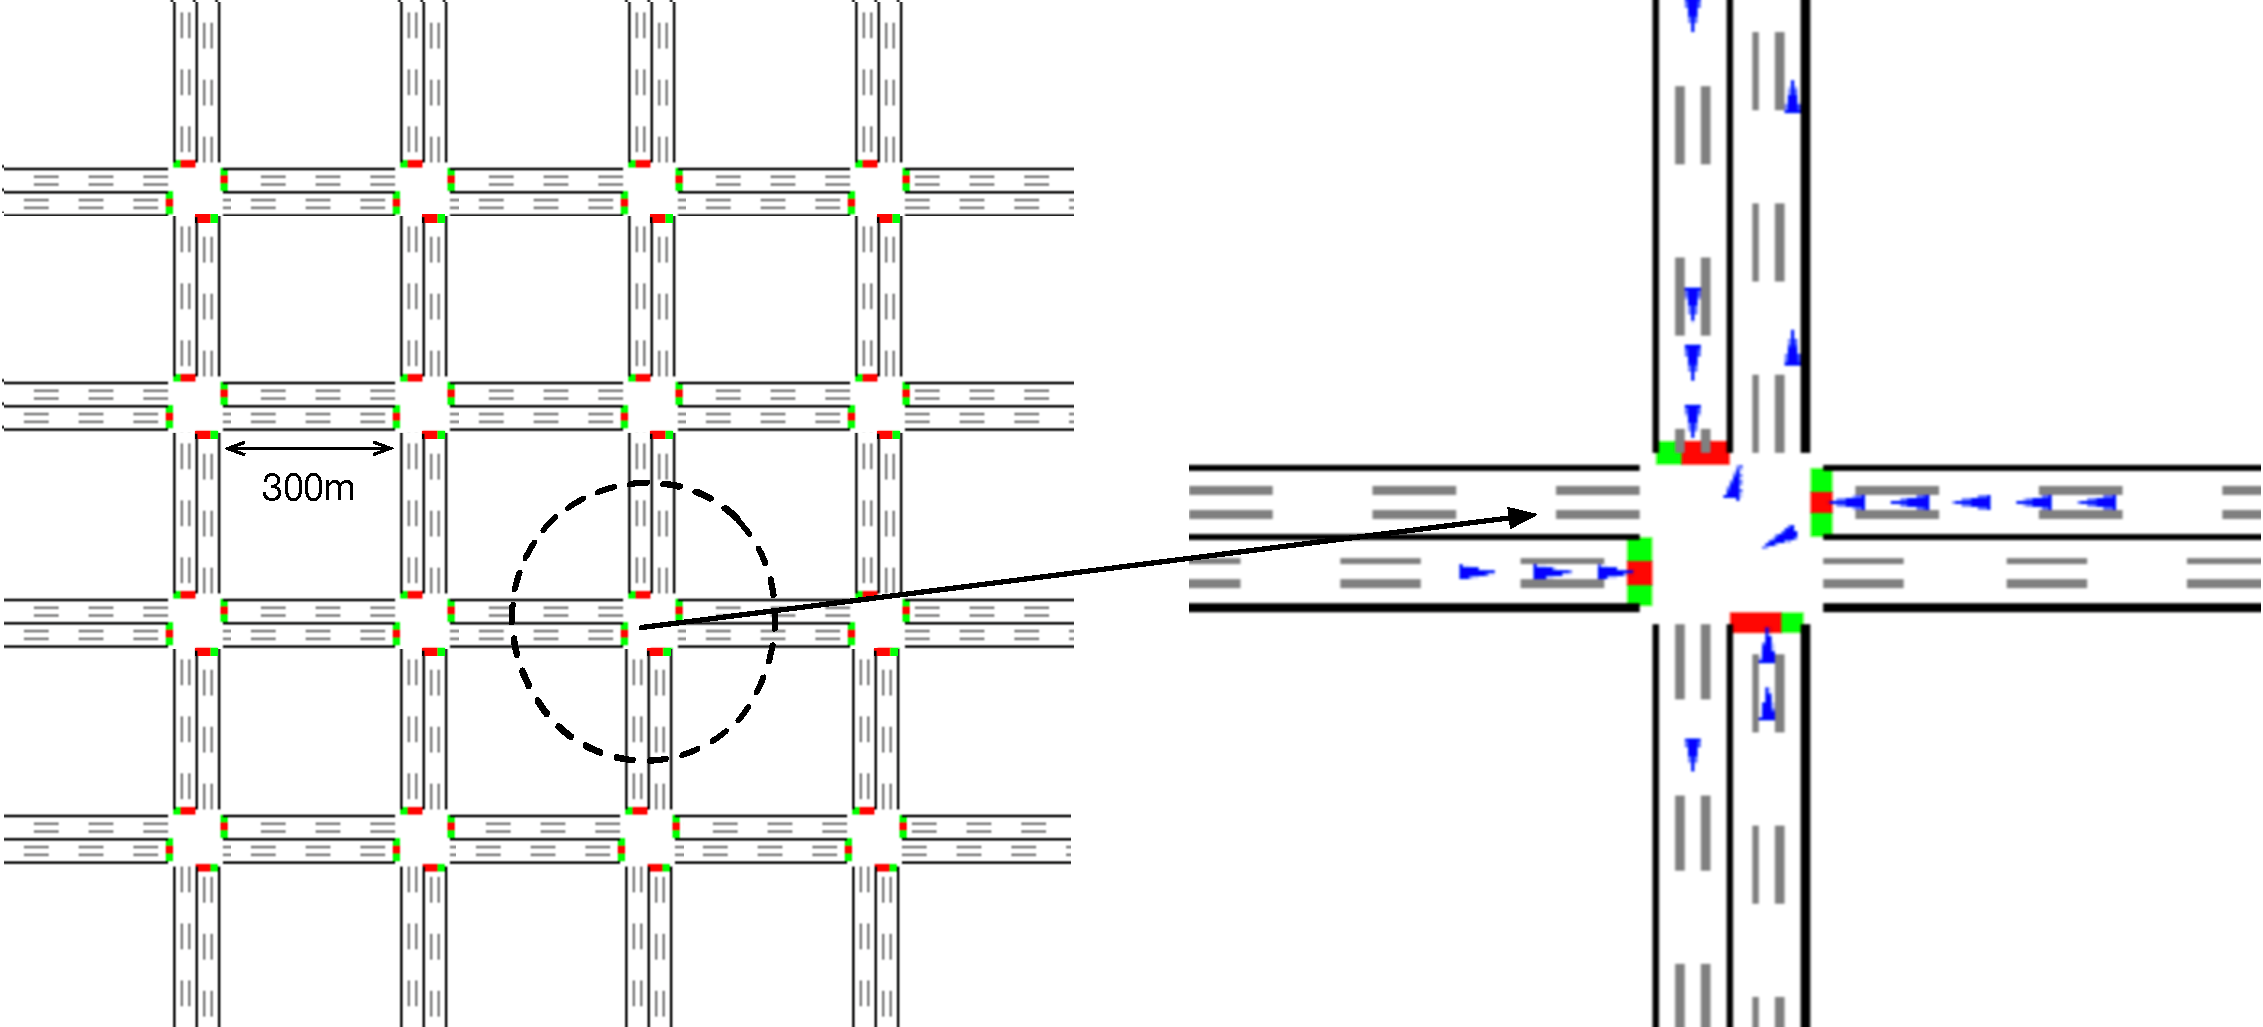
\includegraphics[width=0.5\textwidth]{figures/road_net.pdf} \vspace{-2mm}
\caption{$4\times4$ road network.}\vspace{-2mm}
\label{fig:net}
\end{figure}

% \begin{figure}[htbp]
% \centering
% 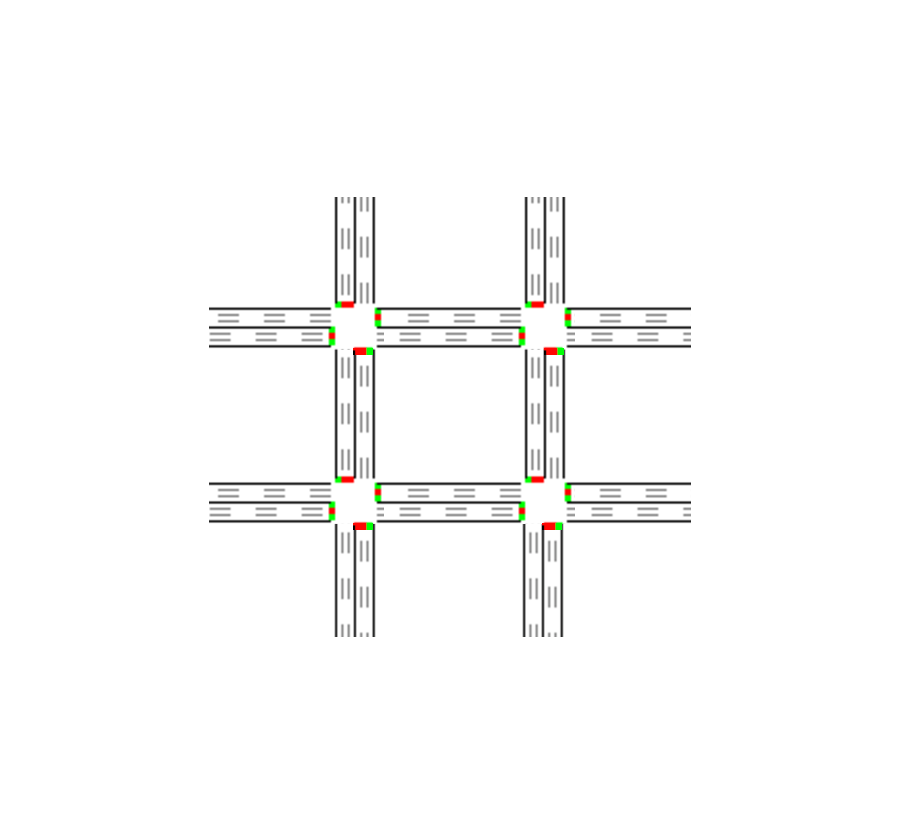
\includegraphics[width=0.25\textwidth]{figures/road_net_2_2.pdf} \vspace{-2mm}
% \caption{$2\times2$ road network.}\vspace{-2mm}
% \label{fig:net2}
% \end{figure}
% There are flat and peak (fluctuated) patterns for traffic flows and data are statistically synthesized from real-world traffic in Jinan and Hangzhou.
% \begin{itemize}
% 	\item Flat  \& Fluctuated
% 	% \item Undersaturated \& Oversaturated
% \end{itemize}
\item Real-world data. We use real traffic data in Manhattan, New York City. Detailed statistics are shown in Table~\ref{tab:real-table} and the road network of Manhattan is demonstrated in Figure~\ref{fig:road-net}. Note that the manhattan dataset contains signalized 2510 traffic lights.\\

\begin{figure}[t!]
  \centering
        % \begin{subfigure}[t]{.2\textwidth}
        %  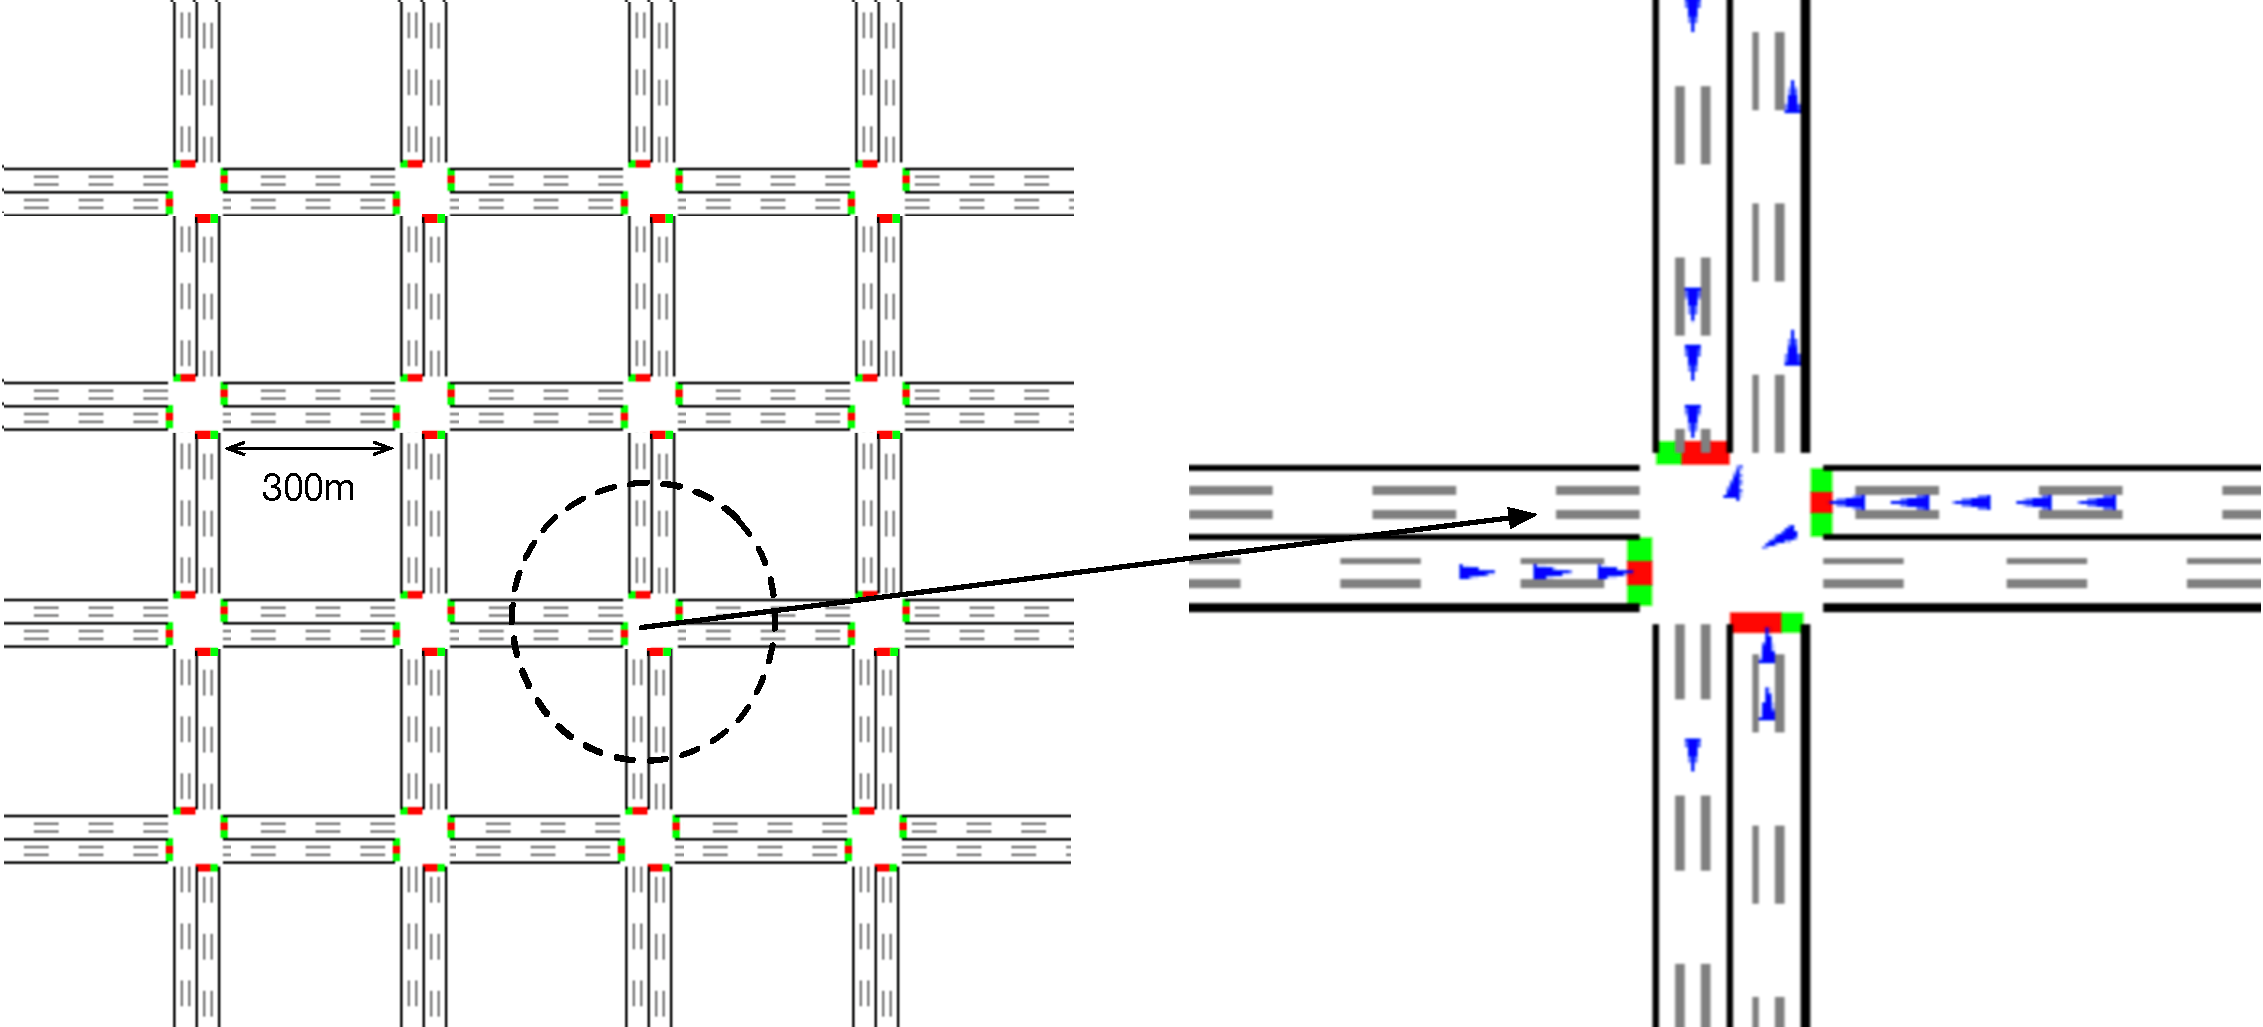
\includegraphics[width=\textwidth]{figures/road_net.pdf}
        %         \caption{$4\times4$ road network.}
        %         % \vspace{-.1in}
        %         \label{fig:manhattan}
        % \end{subfigure}
        % \hfill
        \begin{subfigure}[t]{.2\textwidth}
         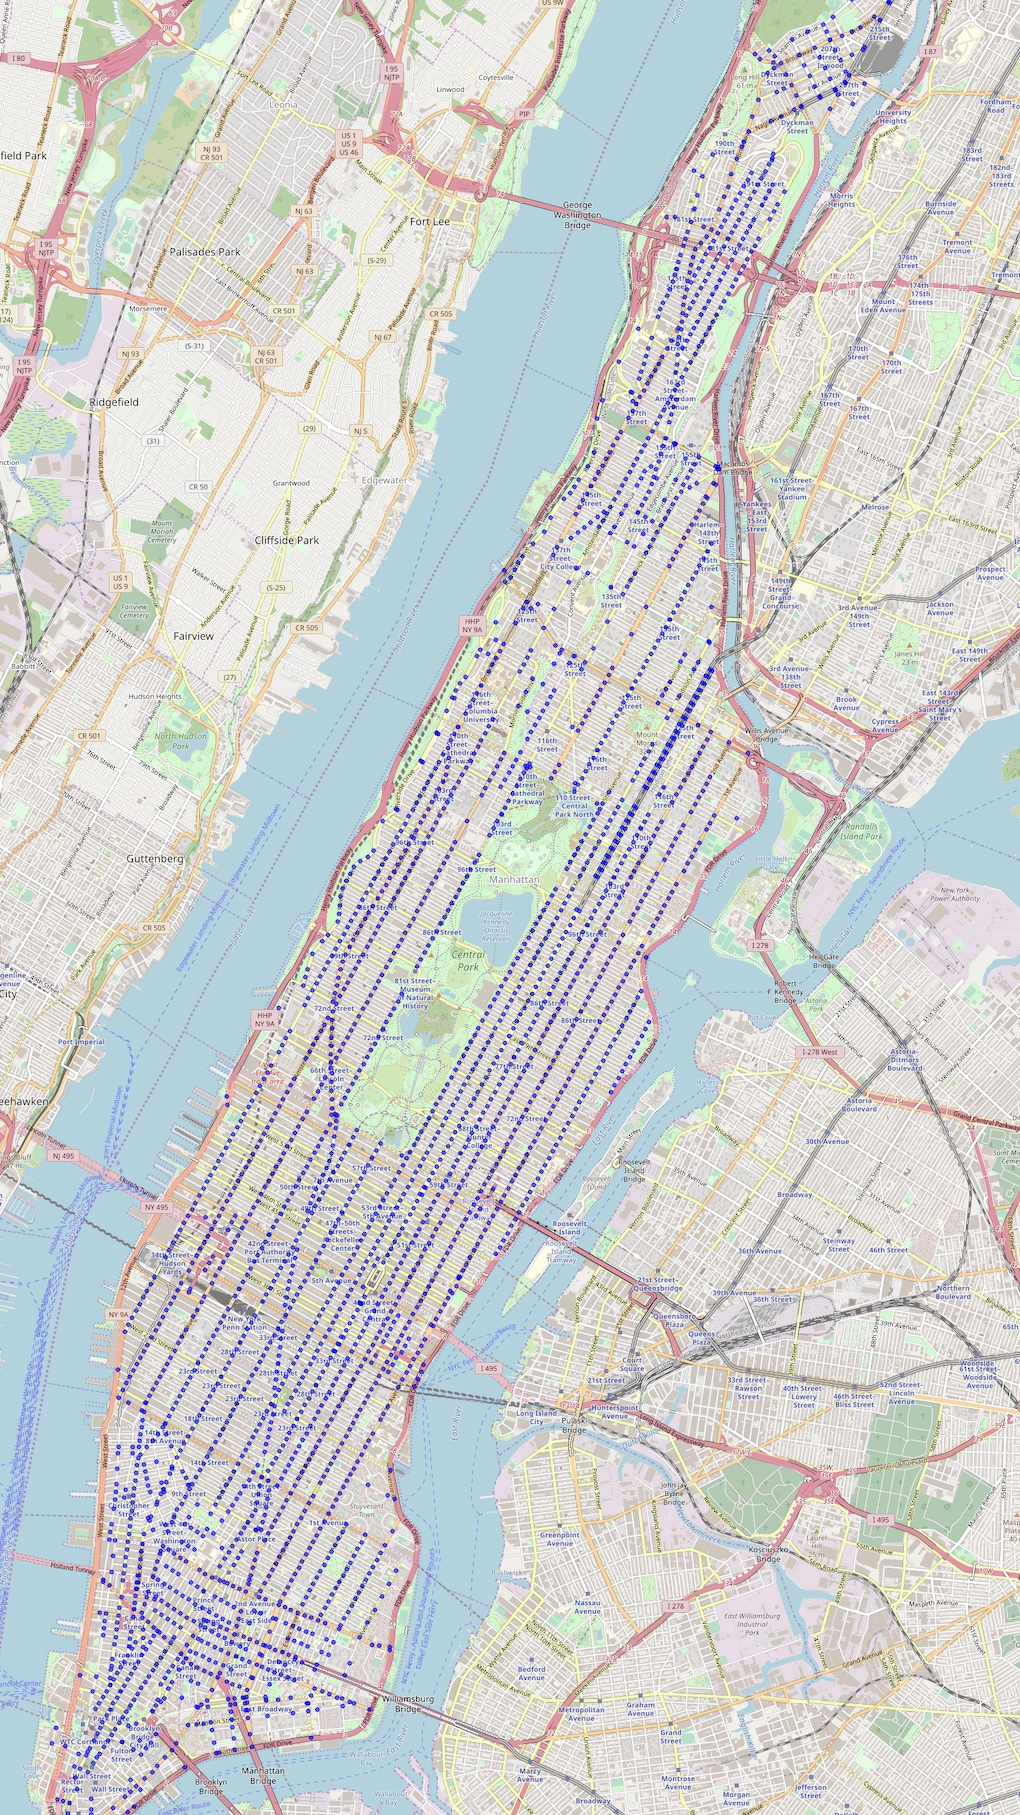
\includegraphics[width=\textwidth]{figures/IMG_2711.jpg}
                \caption{Manhattan}
                % \vspace{-.1in}

        \end{subfigure}
        \hfill
            \begin{subfigure}[t]{.2\textwidth}
         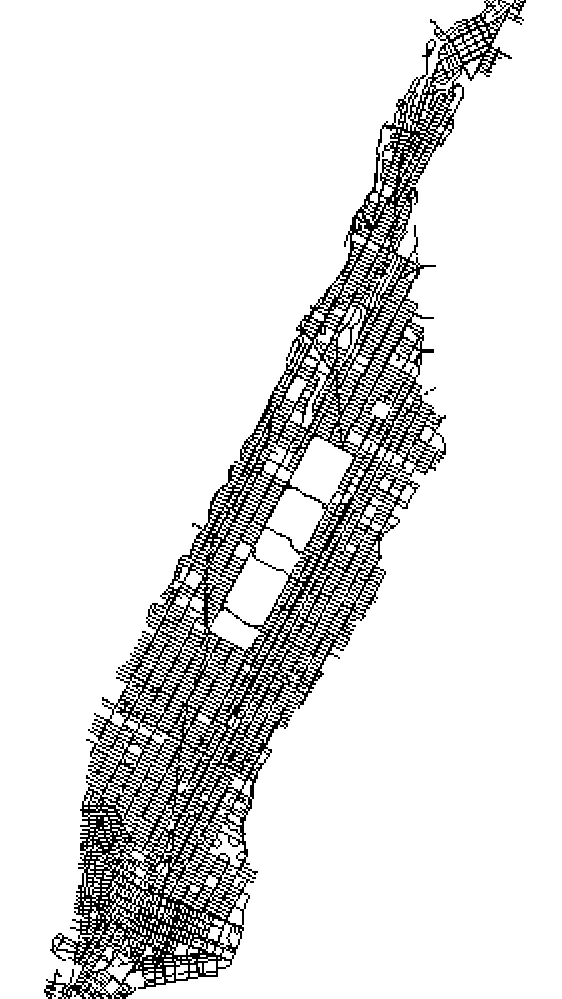
\includegraphics[width=\textwidth]{figures/IMG_2712.jpg}
                \caption{Manhattan in SUMO}
                % \vspace{-.1in}
        \end{subfigure}
        %         \begin{subfigure}[t]{0.45\textwidth}
        %  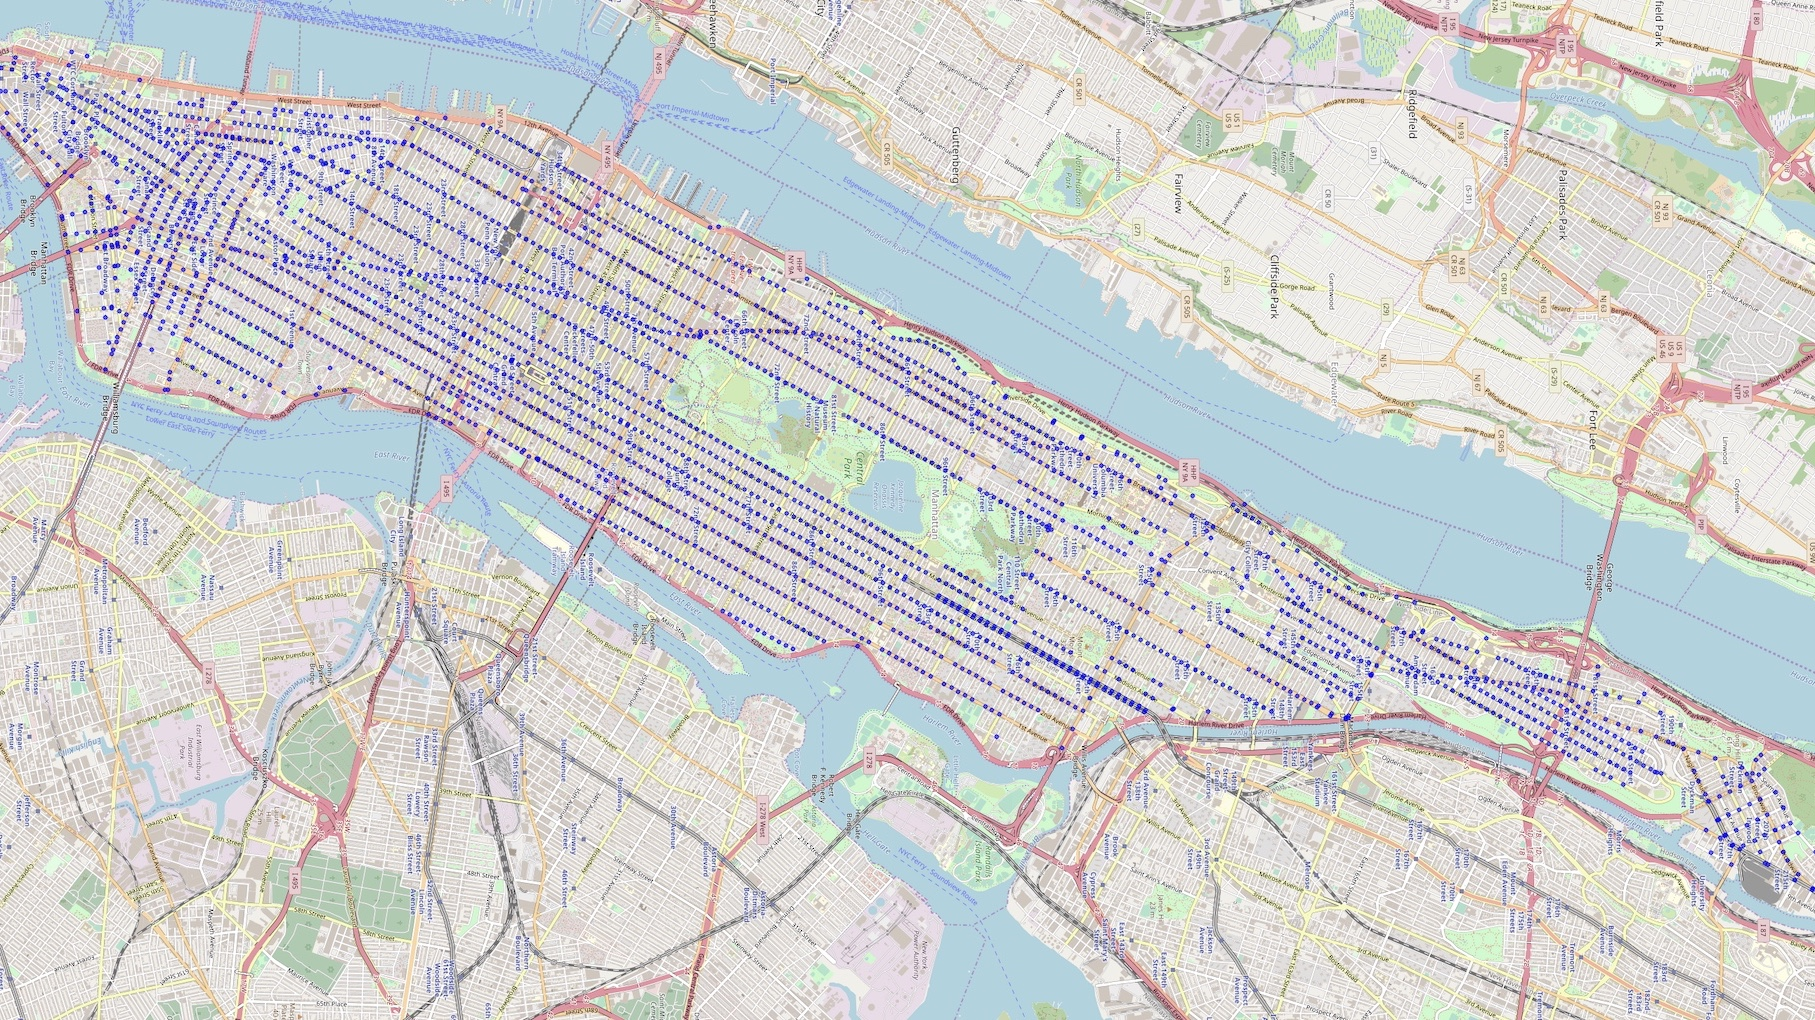
\includegraphics[width=\textwidth,height=0.13\textheight]{figures/manhattan-rotate.jpg}
        %         \caption{Manhattan}
        %         % \vspace{-.1in}

        % \end{subfigure}
        % \hfill
        %     \begin{subfigure}[t]{0.45\textwidth}
        %  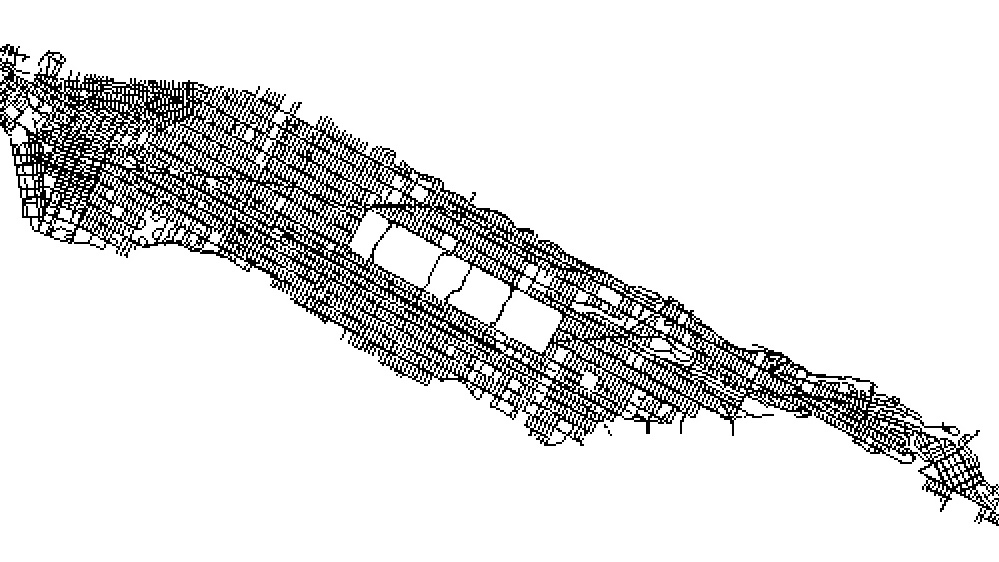
\includegraphics[width=\textwidth,height=0.13\textheight]{figures/manhattan-sumo-rotate.jpg}
        %         \caption{Manhattan in SUMO}
        %         % \vspace{-.1in}
        % \end{subfigure}
%   \subfigure[Config 1]{\label{fig:MFD_700_03} 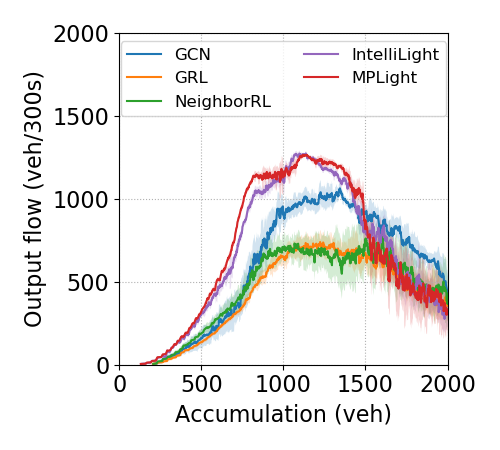
\includegraphics[width=0.3\textwidth]{figures/anon_4_4_700_03_synthetic.png}}
%   \subfigure[Config 2]{\label{fig:MFD_700_06} 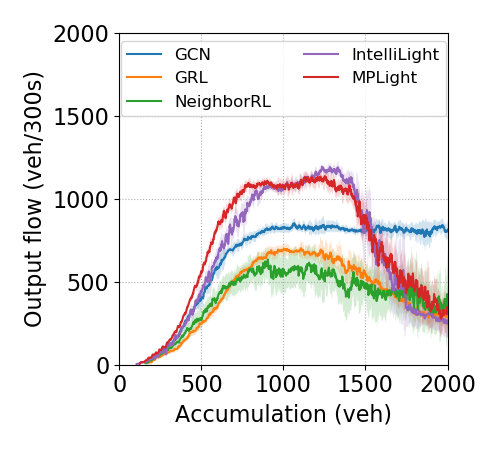
\includegraphics[width=0.3\textwidth]{figures/anon_4_4_700_06_synthetic.png}}
%   \subfigure[Config 3]{\label{fig:MFD_750_03} 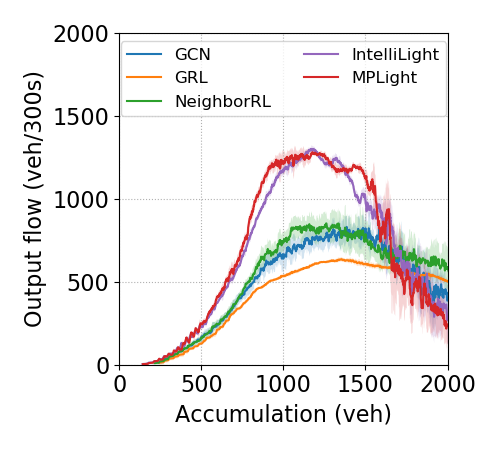
\includegraphics[width=0.3\textwidth]{figures/anon_4_4_750_03_synthetic.png}}
%   \subfigure[Config 4]{\label{fig:MFD_750_06} 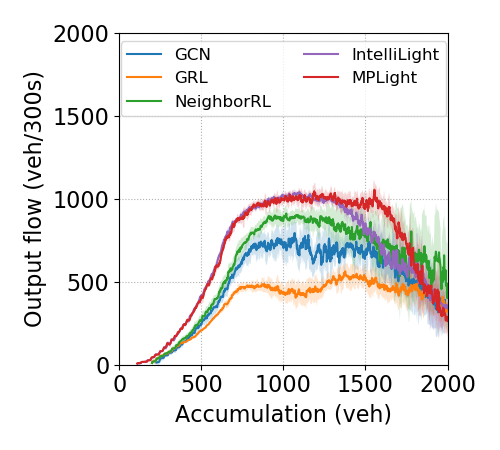
\includegraphics[width=0.3\textwidth]{figures/anon_4_4_750_06_synthetic.png}}
  \caption{Road network of Manhattan in our experiments.}
  \label{fig:road-net}
\end{figure}
% \todo{yuanhao}
% and make the manhattan figure beatiful
\end{itemize}
% \begin{figure*}[t!]
%   \begin{tabular}{cc}
%     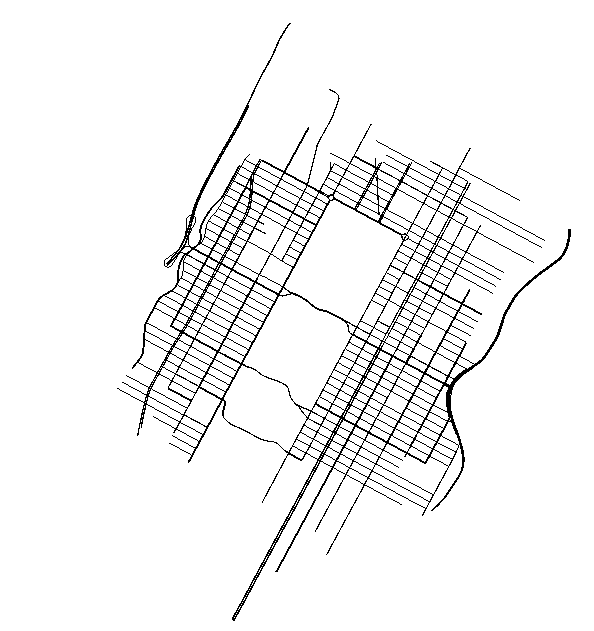
\includegraphics[width=0.5\textwidth,height=0.25\textheight]{figures/manhattan_1km.png} &
% 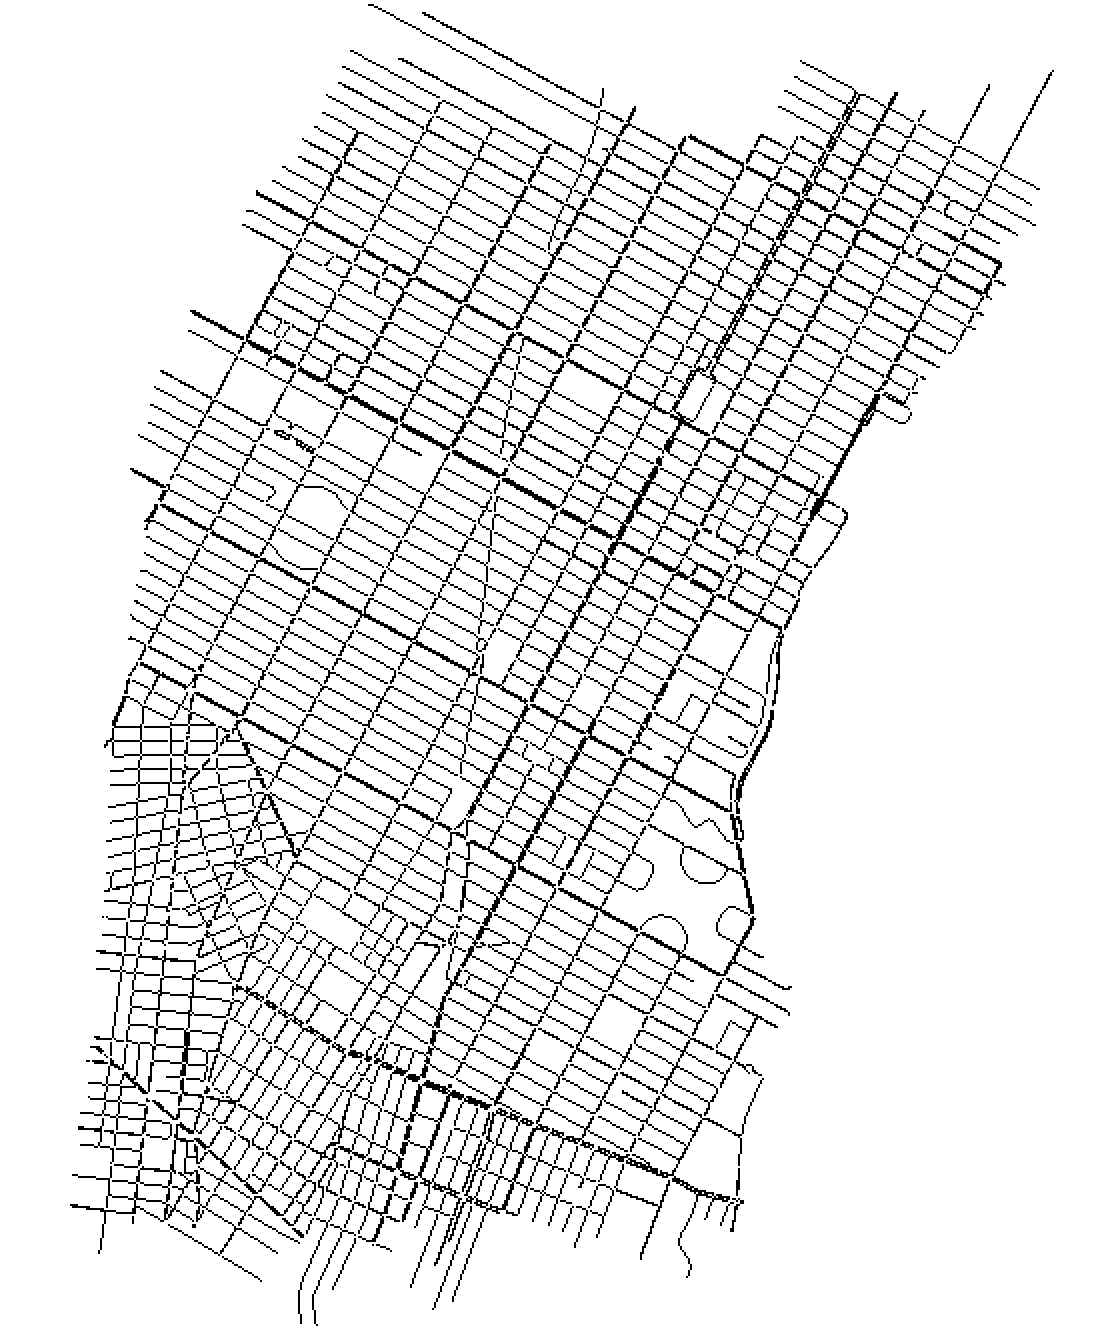
\includegraphics[width=0.5\textwidth,height=0.25\textheight]{figures/manhattan_all.png} \\
% (a) manhattan\_1km & \multicolumn{1}{c}{(b) manhattan\_all} \\
%     \end{tabular}
% \\
% \caption{Manhattan}
% \end{figure*}

\begin{table}[h!]
\begin{center}
% \vspace{-3mm}
\caption{Four configurations of synthetic traffic data}
\label{tab:synthetic-table}
\begin{tabular}{ccc}
\toprule
Config        & \begin{tabular}[c]{@{}c@{}}Demand Pattern \end{tabular}  & \begin{tabular}[c]{@{}c@{}}Arrival rate (vehicles/s)\end{tabular}    \\ \midrule
1 & Flat           & \multirow{2}{*}{0.388}  \\\cmidrule(lr){1-2}
2 & Peak           &         \\ \midrule
3 & Flat           & \multirow{2}{*}{0.416}   \\\cmidrule(lr){1-2}
4 & Peak           &               \\ \midrule
\end{tabular}
% \\\footnotesize{$^{*}$ For illustrations about two patterns, see Figure~\ref{fig:Traffic-direc-pattern-1} and~\ref{fig:Traffic-direc-pattern-2} in Addendum.}\\
\vspace{-3mm}
\end{center}
\end{table}

% \todo{Weihua}

\begin{table}[t]
\caption{Data statistics of the real-world dataset}\label{tab:real-table}
\centering
% \hspace{-.3in} 
\begin{tabular}{cccccc}
\toprule
\multirow{2}{*}{Dataset}  & \multicolumn{4}{c}{Arrival rate (vehicles/h)}  & \multirow{2}{*}{\begin{tabular}[c]{@{}c@{}}\# of \\ Intersections\end{tabular}}\\
                           & Mean         & Std         & Max       & Min    &    \\\midrule
\begin{tabular}[c]{@{}c@{}} Manhattan \end{tabular} &   7576     &  586     &   4272     &  8220  & 2510    \\ 
\bottomrule
\end{tabular}

\end{table}


\subsubsection{Compared Methods}

\begin{itemize}
\item \FT~\cite{koonce2008traffic}: a policy gives a fixed cycle length with a predefined green ratio split among all the phases. It is widely used for steady traffic.
% \item \Greenwave~\cite{Roess2011t}: the optimal solution to control signals on the arterial with uni-directional small traffic flows. All the intersections share the same cycle length and the green ratio split, but with different offsets to form the green wave.
\item \Maxpressure~\cite{varaiya2013max}: the max pressure control selects the phase as green, in order to maximize the pressure according to the upstream and downstream queue length. It is the state-of-the-art control method in the transportation field for signal control in the network level.
\item \NIPS~\cite{van2016coordinated}: a deep Q-learning algorithm for coordinated traffic signal control. Specifically, the transfer planning and the max-plus coordination algorithm are employed for large-scale coordination.
\item \GCN~\cite{nishi2018traffic}: an RL-based traffic signal control method that employs a graph convolutional neural (GCN) network for representing geometric features among multiple intersections. 
\item \NeighborRL~\cite{arel2010reinforcement}: a multi-agent deep Q-learning algorithm that feeds the model with both its own and its neighbors' observations to implement network-level cooperation.
\item \Deeplight~\cite{wei2018intellilight}: the state-of-the-art deep Q-learning method to control signals in a single intersection. A phase selector and a memory palace are introduced for more efficient learning. 
% \item MARLIN~\cite{} 
\end{itemize}

\subsubsection[wide,noitemsep,topsep=0pt]{Evaluation Metrics}
We select the following two representative measures to evaluate different methods.
\begin{itemize}
\item \textbf{Travel time.} Average travel time of all vehicles spent in the system is the most frequently used measure to evaluate the performance of the signal control method in the transportation field.
\item \textbf{Throughput.} It is defined as the number of trips completed by vehicles and can reflect the effectiveness of the model combined with travel time.
\end{itemize}



\subsection{Performance Comparison (RQ1)}
In Table~\ref{tab:synthetic_performance}, we show the performance of transportation methods as well as Deep Reinforcement models on synthetic traffic data in Table. We can obviously discover that the proposed \PressLight consistently outperforms all the other methods in the four different scenarios, leading to both the least time cost of passengers and the maximum utilization of the road resource. The maximum reduction of travel time by \PressLight is $21.86\%$ over the second optimal solution \Maxpressure under Config 3, while the maximum enhancement of throughput over the second-best \Deeplight is as high as $13.07\%$ under Config 4.

The advantage of \PressLight over the other transportation and reinforcement learning methods can be attributed to its decent reward design and feedback learning from the environment at the same time. Compared with the other RL methods, \PressLight optimizes the control strategy by reducing the pressure between the entering and exiting lanes. Although the policy of \Maxpressure also depends on the pressure of different phases, there is a large performance margin from \PressLight in either travel time or throughput, since it ignores the assessment of previous action from the environment.

\begin{table*}[htbp]
\centering
\caption{Performance comparison of different methods evaluated in the four configurations of synthetic traffic data. For average travel time, the lower the better while for throughput, the higher the better.}
\label{tab:synthetic_performance}
\begin{tabular}{lcccccccc}
% {p{0.1\textwidth}p{0.07\textwidth}p{0.07\textwidth}p{0.07\textwidth}p{0.07\textwidth}|p{0.07\textwidth}p{0.07\textwidth}p{0.07\textwidth}p{0.07\textwidth}p{0.07\textwidth}}
\toprule
\multirow{2}[3]{*}{Model}&\multicolumn{4}{c}{Travel Time}&\multicolumn{4}{c}{Throughput}\\
\cmidrule(lr){2-5}\cmidrule(lr){6-9}
&Config 1&Config 2&Config 3&Config 4&Config 1&Config 2&Config 3&Config 4\\\midrule
\FT & 573.13 & 564.02 & 536.04 & 563.06 & 3555& 3477 & 3898 & 3556\\ 
\Maxpressure & 361.17 & 402.72 & 360.05 & 406.45 & 4702 & 4324 & 4814 & 4386\\ \midrule
\NIPS & 735.38 & 758.58 & 771.05 & 721.37 & 3122 & 2792& 2962 & 2991\\ 
\GCN & 516.65 & 523.79 & 646.24 & 585.91 & 4275 & 4151 & 3660 & 3695\\
\NeighborRL & 690.87 & 687.27 & 781.24 & 791.44 & 3504 & 3255 & 2863 & 2537\\
\Deeplight & 340.44 & 298.55 & 361.36 & 598.52 & 5097 & 5113 & 5483 & 4475 \\ \midrule
\textbf{\PressLight} & \textbf{309.33} & \textbf{262.50} & \textbf{281.34} & \textbf{353.13} & \textbf{5219} & \textbf{5213} & \textbf{5652} & \textbf{5060}   \\ 
% Improvements &   7.85\%          &  8.13\%           &       5.69\%         &      31.17\%       &   28.58\%          &    58.73\%             \\ 
\bottomrule
\end{tabular}
\end{table*}







% \begin{table}[]
% \begin{tabular}{|l|l|l|l|l|l|l|l|l|}
% \hline
%             & \multicolumn{4}{l|}{travel time}         & \multicolumn{4}{l|}{throughput}     \\ \hline
% config      & 1         & 2        & 3        & 4      & 1         & 2        & 3     & 4    \\ \hline
% FT          & 466.49    & 438.71   & 496.55   & 488.21 & 6924      & 6761     & 7465  & 7355 \\ \hline
% MP          & 353.29    & 450.65   & 516.00   & 531.53 & 7770      & 7704     & 8636  & 8428 \\ \hline
% IRL         & 348.13    & 400.30   & 322.40   & 391.89 & 2793      & 2829     & 4771  & 5045 \\ \hline
% MARLIN-ATSC &           &          &          &        &           &          &       &      \\ \hline
% PressLight  & 192.22    & 277.65   & 207.75   & 294.13 & 4588      & 4126     & 4960  & 5098 \\ \hline
%             & \multicolumn{4}{l|}{travel time}         & \multicolumn{4}{l|}{throughput}     \\ \hline
%             & Manhattan & Hangzhou & Jinan    & LA     & Manhattan & Hangzhou & Jinan & LA   \\ \hline
% FT          & 367.236   & 463.5019 & 428.856  &        & 1714      & 2524     & 5542  &      \\ \hline
% MP          & 486.81    & 386.047  & 410.8139 &        & 2223      & 2875     & 5801  &      \\ \hline
% IRL         &           &          &          &        &           &          &       &      \\ \hline
% MARLIN-ATSC &           &          &          &        &           &          &       &      \\ \hline
% PressLight  &           &          &          &        &           &          &       &      \\ \hline
% \end{tabular}
% \end{table}


% \subsection{Reward Function Study (RQ2)}
\begin{figure}[t!]
  \centering
        \begin{subfigure}[t]{.23\textwidth}
         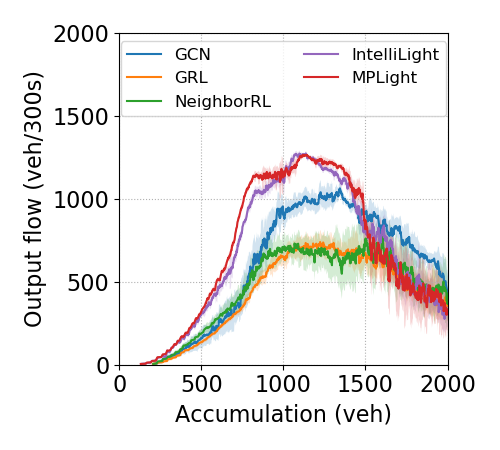
\includegraphics[width=\textwidth]{figures/anon_4_4_700_03_synthetic.png}
                \caption{Config 1.}
                % \vspace{-.1in}
                \label{fig:MFD_700_03}
        \end{subfigure}
        \hfill
        \begin{subfigure}[t]{.23\textwidth}
         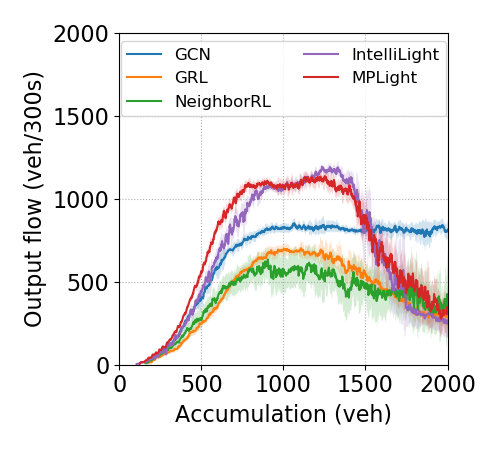
\includegraphics[width=\textwidth]{figures/anon_4_4_700_06_synthetic.png}
                \caption{Config 2.}
                % \vspace{-.1in}
                \label{fig:MFD_700_06}
        \end{subfigure}
        \hfill
        \begin{subfigure}[t]{.23\textwidth}
         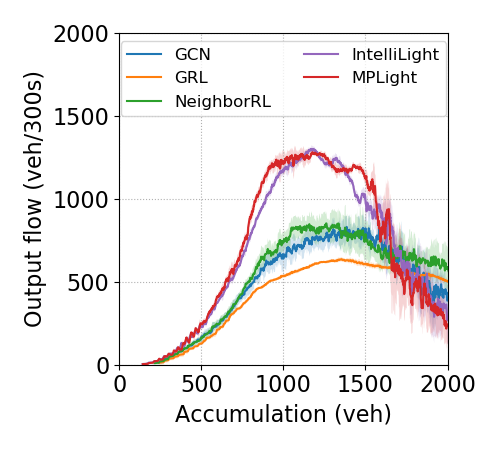
\includegraphics[width=\textwidth]{figures/anon_4_4_750_03_synthetic.png}
                \caption{Config 3.}
                % \vspace{-.1in}
                \label{fig:MFD_750_03}
        \end{subfigure}
        \hfill
        \begin{subfigure}[t]{.23\textwidth}
         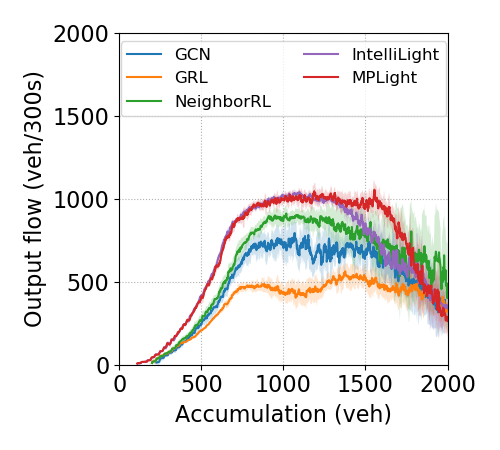
\includegraphics[width=\textwidth]{figures/anon_4_4_750_06_synthetic.png}
                \caption{Config 4.}
                % \vspace{-.1in}
                \label{fig:MFD_750_06}
        \end{subfigure}
  \caption{The macroscopic fundamental diagrams (MFD) of network traffic controlled by RL methods under four different configurations. It shows the relation between the total number of vehicles (accumulation) on the road and the rate at which trips reach their destinations (output flow). The higher the output flow, the better the signal control method.}
  \label{fig:MFD_analysis}
\end{figure}

\subsection{Road Resource Utilization Study (RQ2)}
In the transportation area, Macroscopic Fundamental Diagram (MFD) is used to reflect the relation between the vehicle accumulation in network and outflow of the network. As is shown in Figure~\ref{fig:MFD_analysis}, the horizontal axis is the total vehicle in the network, and the vertical axis is the total vehicles that complete their trips in the network. When the vehicle accumulation in the network is less than the sweet spot, the outflow of the network increases with the increase of the accumulation and then arrives at the
optimal throughput. If the vehicle accumulation is more than the sweet spot, the outflow decreases with the increase of the accumulation. Given the output flows of a network, a smaller accumulation indicates fewer vehicles in the network, indicating a better control strategy. Similarly, given the accumulations in a network, a higher output flow indicates the better control strategy. In Figure~\ref{fig:MFD_analysis},  \PressLight presents a higher output flow value given the same vehicle accumulation.

%Figure 4 plots the output flow and the network accumulation, it could be verified that the network present a fundamental diagram for different signal settings, i.e., the output flow at first increases as the accumulaiton grows, after a `sweet-spot', further accumulation will decrease the output. As we can see, that \PressLight is able to present a higher output flow value given the same vehicle accumulation and the `sweet-spot' of \PressLight is more upper left compared with other methods.

% Network infrastructure shows a property of MFD\\
% When demand conditions are steady, traffic flow streams on long homogeneous roads exhibit reproducible relations between their average flows and densities that engineers call “fundamental diagrams”. It has been recently proposed that entire city neighborhoods must also exhibit similar macroscopic fundamental diagrams (MFD) connecting the total number of cars on the road at any given time (the accumulation) with the rate at which trips reach their destinations (the output). It has also been proposed that the MFD of neighborhoods that are not too big should be independent of where people are going (the neighborhoods “origin-destination table”); i.e., the MFD should be a property only of the network infrastructure. Daganzo (2007) explains why.



% \subsection{Convergence Analysis}
\subsection{Impact of Parameter Sharing on Model Learning (RQ3)}
To investigate the impact of parameter sharing in model learning, we compare the performance of our RL agent design with and without parameter sharing under synthetic traffic. As is shown in Figure~\ref{fig:convergence}, parameter sharing enables our model to converge faster, which verifies the effectiveness of parameter sharing for controlling traffic signals.
% \begin{table}[htbp]
% \centering
% \caption{Number of episodes for different models to converge.}
% \label{tab:convergence}
% \begin{tabular}{ccccc}
% \toprule
% Model& config.1 & config.2 & config.3 & config.4 \\\midrule
% N model               & 19       & 30       & 93       & 112      \\\midrule
% One model             & \bf 7        & \bf 20       & \bf 77       & \bf 85\\\bottomrule      
% \end{tabular}
% \end{table}
% CONVERGE FIGURE{\color{red}todo-weihua}

\begin{figure}[htbp]
\centering
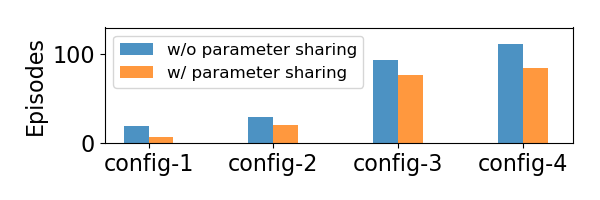
\includegraphics[width=0.5\textwidth]{figures/ccc_converge_ijcai.png}

\caption{Number of episodes for models to converge.}
\label{fig:convergence}
\end{figure}

% Figure 3 (number of trips ended as time)

% {\color{red} Can PressLight assure a network's vehicle accumulation remains as close as possible to the "sweet-spot" value?}

% No. But it is trying as best to maintain the sweet point value as long as possible if the traffic volume is increasing consistently, see (b).


% This result is promising for society because something simple and cheap (minimize delta q) can have a significant and verifiable benefit.

\subsection{Scalability Analysis (RQ4)}
In this part, we turn to experiments on real-world data. We evaluate our proposed method with other baselines under Manhattan, New York City, where there are over 2500 signalized intersections. The problem of such a large scale is usually difficult to deal with through conventional methods in the transportation field.

As shown in Table~\ref{tab:large-scale}, our method achieves the best performance over other baseline methods on both travel time and throughput. It should be noted that two methods including \NIPS and \NeighborRL can not be compared as they are unable to scale to large networks due to high complexity and computational costs. On the contrary, our proposed method \PressLight can handle traffic signal control for thousands of lights effectively and efficiently

% \begin{figure}[htbp]
% \centering
% 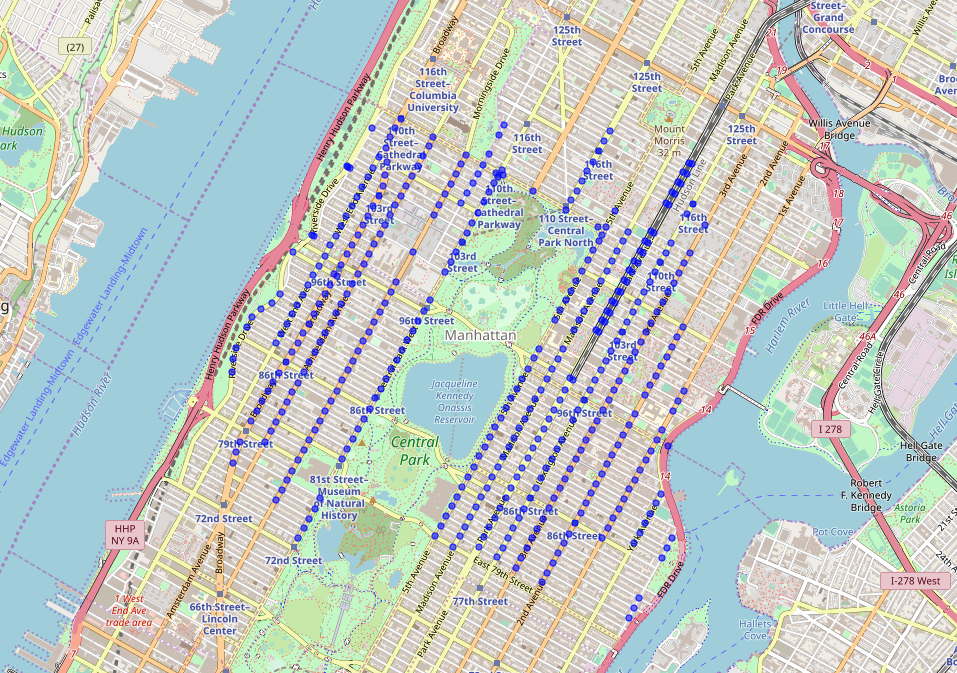
\includegraphics[width=0.5\textwidth]{figures/manhattan_1km_real.png} \vspace{-2mm}
% \caption{manhattan 1km real}\vspace{-2mm}
% \label{fig:pressure}
% \end{figure}


% \begin{figure}[htbp]
% \centering
% \includegraphics[width=0.5\textwidth]{figures/manhattan_all_real.png} \vspace{-2mm}
% \caption{manhattan all real}\vspace{-2mm}
% \label{fig:pressure}
% \end{figure}




\begin{table}[htbp]
\caption{Performance of different methods on Manhattan.}
\begin{center}
\begin{tabular}{lcc}
\toprule
Model   & Travel Time&Throughput            \\\midrule
\FT         &  193.66        &     7398         \\
\Maxpressure&  133.72&              7620        \\\midrule
\NIPS       &   -$^{*}$        & -$^{*}$          \\
\GCN        &  139.01      &    5436            \\
\NeighborRL &  -$^{*}$       &     -$^{*}$           \\
\Deeplight  & 162.81   &   6816   \\\midrule
\PressLight &\bf 126.55&\bf8154\\\bottomrule   
\end{tabular}
\label{tab:large-scale}
\\
% \footnotesize{$^{*}$No result as **** can not scale up to thousands of intersections in New York's road network.}
\end{center}
No result as \NIPS and \NeighborRL can not scale up to thousands of intersections in New York's road network.
\end{table}



\section{Conclusion}

In this chapter, we propose a deep reinforcement learning method to tackle the problem of city-level traffic signal control. Specifically, we use theoretically guaranteed reward design and knowledge sharing to maximize the total throughput of the controlled region. We are the first to evaluate the RL-based traffic signal control methods in a real-world scenario with thousands of traffic lights. Our proposed method has shown its ability in delivering strong performance, generalization and its scalability.

We also acknowledge the limitations of our current approach and would like to point out a few possible future directions. First, we consider the scenario where only vehicles exist. However, in the real world, patterns of pedestrians and non-motorized vehicles, which can influence traffic signal control significantly, need to be taken into account. Second, although allocating a shared agent for all intersections achieves satisfactory control in the large-scale road network, more elaborate design for coordination and cooperation among neighboring intersections might further improve performance. Lastly, all experiments are currently carried out on a simulation platform. A field study would be an important future step for our model to get real-world feedback and for us to validate the proposed reinforcement learning approach.

  
